\documentclass[10pt,letterpaper]{article}
\usepackage[margin=0.55in]{geometry}
\usepackage[T1]{fontenc}
\usepackage{lmodern}
\usepackage{microtype}
\usepackage{enumitem}
\setlist{nosep}
\usepackage{amsmath,amssymb}
\usepackage{booktabs}
\usepackage{tabularx}
\usepackage{xcolor}
\usepackage[hidelinks]{hyperref}
\usepackage{tikz}
\usetikzlibrary{shapes.geometric,arrows.meta,positioning}
\usepackage{titlesec}
\usepackage{fancyhdr}

\definecolor{accent}{HTML}{1F5FA8}
\definecolor{aicol}{HTML}{C77700}
\definecolor{codecol}{HTML}{1F5FA8}
\definecolor{humcol}{HTML}{2C7A2C}
\definecolor{alert}{HTML}{B00020}

\setlength{\parindent}{0pt}
\setlength{\parskip}{2.5pt}
\setlength{\tabcolsep}{3pt}
\renewcommand{\arraystretch}{1.08}
\setlength{\emergencystretch}{2em}

\titleformat{\section}{\large\bfseries\color{accent}}{\thesection.}{0.5em}{}[{\color{accent!40}\titlerule[0.4pt]}]
\titlespacing*{\section}{0pt}{8pt}{4pt}

\pagestyle{fancy}
\fancyhf{}
\renewcommand{\headrulewidth}{0.3pt}
\lhead{\scriptsize\textcolor{gray}{Auditable Covenant Compliance -- Take-Home Brief}}
\rhead{\scriptsize\textcolor{gray}{Page \thepage\ of 4}}
\setlength{\headheight}{12pt}
\setlength{\footskip}{14pt}

\newcommand{\ct}[1]{\texttt{\small #1}}
\newcolumntype{Y}{>{\raggedright\arraybackslash}X}
\newcommand{\tabsize}{\footnotesize}

\begin{document}

{\raggedright\Large\bfseries\color{accent} Auditable Covenant Compliance: compile the contract once, compute it deterministically every quarter\par}
\vspace{-3pt}{\color{accent}\rule{\linewidth}{1.2pt}}

\textbf{Domain:} commercial-loan financial-covenant monitoring. \textbf{Jurisdiction:} US credit agreements (NY law), using public EDGAR Exhibit~10 filings and 10-Q/10-K financials. For another jurisdiction the definitions and amendment conventions change; the architecture does not. \textbf{All cost figures below are my estimates, not sourced data, and every example is synthetic.}

\textbf{What surprised me.} The ratio math is trivial (net debt / EBITDA). The risk is the \emph{definition}: ``Consolidated EBITDA'' differs per agreement, add-backs are capped, cash netting is capped, thresholds step down, and amendments silently redefine terms. A template fails because every agreement is bespoke, and one LLM call that returns the ratio cannot be audited.

%------------------------------------------------------------------
\section{Problem statement}
\begin{tabularx}{\linewidth}{@{}l Y@{}}
\toprule
\tabsize\textbf{Who} & \tabsize Covenant-monitoring analysts in credit administration at a mid-market lender; the credit officer who signs findings. \\
\midrule
\tabsize\textbf{Task} & \tabsize Each quarter, per borrower: find the financial covenants in a 100--300 page agreement, apply all amendments, extract inputs from the financials and compliance certificate, recompute ratios under the contract's own definitions, flag breaches and thin headroom. \\
\midrule
\tabsize\textbf{Frequency} & \tabsize Quarterly (some monthly). About 400 borrowers gives about 1,600 tests a year. Certificates are due about 45 days after quarter end, so about 60\% of tests land in one 3-week window. \\
\midrule
\tabsize\textbf{Cost today} & \tabsize About 4.5\,h per test, about 7,200\,h a year, roughly 4 FTE, about \$650K a year at \$90/h loaded. The larger cost is a breach found late (lost early-intervention leverage) or a false pass. \\
\midrule
\tabsize\textbf{Out of scope} & \tabsize Waiver and reservation-of-rights decisions, legal notices, pricing and rating, non-financial covenants, equity-cure modelling (flagged only), pro-forma acquisition adjustments, any real client data. The system gives decision support, not legal advice. \\
\bottomrule
\end{tabularx}

%------------------------------------------------------------------
\section{Solution design}
\textbf{Core idea.} The LLM compiles each agreement version once into a typed, human-approved \ct{CovenantSpec}. A deterministic engine then executes that spec every quarter. The LLM never touches a number that enters a ratio without a verified source span. \textbf{Why AI at all:} definitions are bespoke natural language with cross-references (``as amended by Amendment No.~2''); that is the one step regex and templates cannot do.

\begin{center}
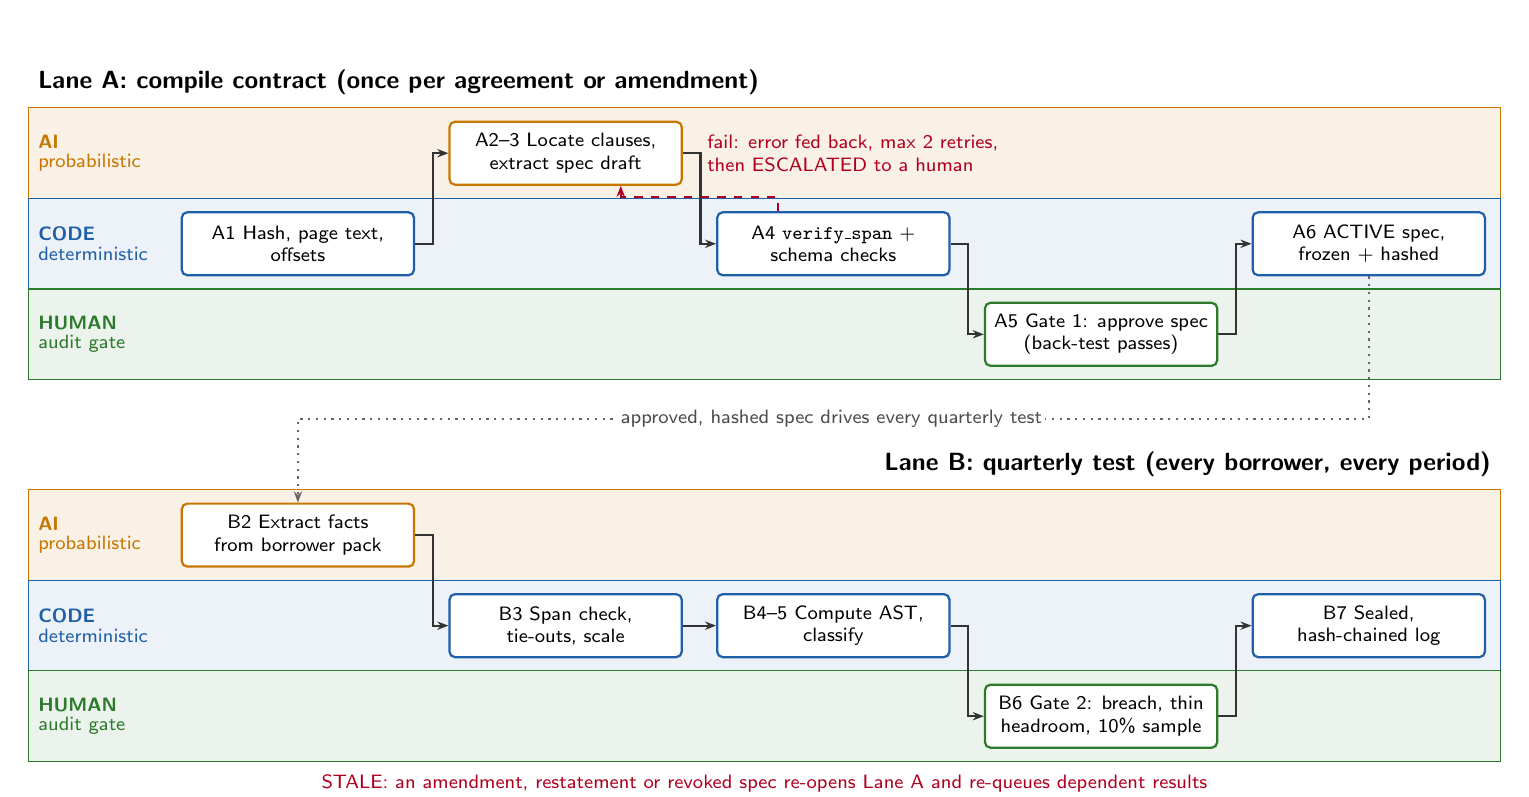
\begin{tikzpicture}[
  x=1cm,y=1cm,
  box/.style={draw,rounded corners=2pt,fill=white,line width=0.8pt,minimum width=2.95cm,minimum height=0.8cm,
              align=center,font=\scriptsize\sffamily,inner sep=2pt},
  aibox/.style={box,draw=aicol},
  codebox/.style={box,draw=codecol},
  humbox/.style={box,draw=humcol},
  arr/.style={-{Stealth[length=4pt]},line width=0.8pt,draw=black!80},
  retry/.style={-{Stealth[length=4pt]},line width=0.8pt,dashed,draw=alert},
  spec/.style={-{Stealth[length=4pt]},line width=0.8pt,dotted,draw=black!60},
  lanelabel/.style={font=\scriptsize\sffamily,align=left,anchor=west,inner sep=2pt}
]
\newcommand{\lanes}[4]{%
  \fill[aicol!10]   (0,#1) rectangle (18.7,#1-1.15);   \draw[aicol]   (0,#1) rectangle (18.7,#1-1.15);
  \fill[codecol!8]  (0,#1-1.15) rectangle (18.7,#1-2.3); \draw[codecol] (0,#1-1.15) rectangle (18.7,#1-2.3);
  \fill[humcol!9]   (0,#1-2.3) rectangle (18.7,#1-3.45); \draw[humcol]  (0,#1-2.3) rectangle (18.7,#1-3.45);
  \node[lanelabel,text=aicol]   at (0.05,#1-0.575) {\textbf{AI}\\[-1pt]probabilistic};
  \node[lanelabel,text=codecol] at (0.05,#1-1.725) {\textbf{CODE}\\[-1pt]deterministic};
  \node[lanelabel,text=humcol]  at (0.05,#1-2.875) {\textbf{HUMAN}\\[-1pt]audit gate};
  \node[anchor=south #3,font=\small\sffamily\bfseries] at (#4,#1+0.04) {#2};
}
% Lane A (top at y=0)
\lanes{0}{Lane A: compile contract (once per agreement or amendment)}{west}{0}
\node[codebox] (a1) at (3.425,-1.725) {A1 Hash, page text,\\offsets};
\node[aibox]   (a2) at (6.825,-0.575) {A2--3 Locate clauses,\\extract spec draft};
\node[codebox] (a3) at (10.225,-1.725) {A4 \texttt{verify\_span} +\\schema checks};
\node[humbox]  (a4) at (13.625,-2.875) {A5 Gate 1: approve spec\\(back-test passes)};
\node[codebox] (a5) at (17.025,-1.725) {A6 ACTIVE spec,\\frozen + hashed};
\foreach \s/\t in {a1/a2,a2/a3,a3/a4,a4/a5}{\draw[arr] (\s.east) -- ++(0.225,0) |- (\t.west);}
\draw[retry] ([xshift=-0.7cm]a3.north) -- ++(0,0.175) -| ([xshift=0.7cm]a2.south);
\node[font=\scriptsize\sffamily,text=alert,anchor=west,align=left] at (8.5,-0.575) {fail: error fed back, max 2 retries,\\then ESCALATED to a human};
% Lane B (top at y=-4.85)
\lanes{-4.85}{Lane B: quarterly test (every borrower, every period)}{east}{18.7}
\node[aibox]   (b1) at (3.425,-5.425) {B2 Extract facts\\from borrower pack};
\node[codebox] (b2) at (6.825,-6.575) {B3 Span check,\\tie-outs, scale};
\node[codebox] (b3) at (10.225,-6.575) {B4--5 Compute AST,\\classify};
\node[humbox]  (b4) at (13.625,-7.725) {B6 Gate 2: breach, thin\\headroom, 10\% sample};
\node[codebox] (b5) at (17.025,-6.575) {B7 Sealed,\\hash-chained log};
\foreach \s/\t in {b1/b2,b2/b3,b3/b4,b4/b5}{\draw[arr] (\s.east) -- ++(0.225,0) |- (\t.west);}
% spec feeds lane B
\draw[spec] (a5.south) -- (17.025,-3.95) -- (3.425,-3.95) -- (b1.north);
\node[font=\scriptsize\sffamily,text=black!70,fill=white,inner sep=1pt] at (10.2,-3.95) {approved, hashed spec drives every quarterly test};
\node[font=\scriptsize\sffamily,text=alert,anchor=north] at (9.35,-8.35) {STALE: an amendment, restatement or revoked spec re-opens Lane A and re-queues dependent results};
\end{tikzpicture}
\end{center}
\vspace{-6pt}

\textbf{Knowledge management.} Contract meaning lives in the approved, versioned \ct{CovenantSpec} (code, not weights). Evidence lives in the hashed document store. Bank policy (thin-headroom \%, sampling rate) lives in config. The LLM holds no knowledge the system depends on. \textbf{When knowledge becomes invalid:} (1)~a new amendment or side letter creates a new spec version and supersedes the old; (2)~a borrower restatement flags every result that used the old facts; (3)~a revoked spec flags every dependent result \ct{stale}; (4)~stale results are re-run and a human sees any change in status. Nothing is silently edited.

\textbf{Audit lineage.} Every output walks back: \ct{status} $\rightarrow$ \ct{ratio} $\rightarrow$ \ct{TraceStep} $\rightarrow$ \ct{fact\_id} $\rightarrow$ \ct{SourceSpan(doc\_sha256, page, char\_start:char\_end, quote)} $\rightarrow$ clause text, and via \ct{spec\_hash} to the approving human. An auditor can re-run the sealed inputs through the pinned \ct{engine\_version} and get the same result.

\smallskip
\begin{tabularx}{\linewidth}{@{}p{0.95cm} p{3.4cm} p{2.0cm} Y@{}}
\toprule
\tabsize\textbf{\#} & \tabsize\textbf{State} & \tabsize\textbf{Actor} & \tabsize\textbf{What happens / exit guard} \\
\midrule
\tabsize A1 & \tabsize INGESTED & \tabsize Code & \tabsize Immutable store, SHA-256, per-page canonical text with offsets (OCR flagged with confidence). \\
\tabsize A2 & \tabsize LOCATED & \tabsize AI + code & \tabsize Hybrid retrieval finds covenant section, definitions, amendments; a deterministic cross-reference resolver loops until no capitalised term is undefined. \\
\tabsize A3 & \tabsize EXTRACTED & \tabsize \textbf{AI} & \tabsize Extractor emits a \ct{CovenantSpec} draft; each definition, threshold and constant carries a verbatim quote with page and offsets. \\
\tabsize A4 & \tabsize GROUNDED & \tabsize Code & \tabsize \ct{verify\_span} (quote must equal page text at offsets), schema, no unsourced literals, no cycles, no threshold gaps. Fail: error fed back, max 2 retries, then ESCALATED. \\
\tabsize A5 & \tabsize SPEC\_REVIEW & \tabsize \textbf{Human}, gate 1 & \tabsize Side-by-side PDF highlights and a plain-English rendering of the formula \textbf{generated from the AST by code, not the LLM}. Edits stored as a diff. Credit officer signs; second signer above an exposure limit. \\
\tabsize A6 & \tabsize ACTIVE & \tabsize Code & \tabsize Spec frozen and hashed. Any change is a new version. \\
\bottomrule
\end{tabularx}
\smallskip
\begin{tabularx}{\linewidth}{@{}p{0.95cm} p{3.4cm} p{2.0cm} Y@{}}
\toprule
\tabsize\textbf{\#} & \tabsize\textbf{State} & \tabsize\textbf{Actor} & \tabsize\textbf{What happens / exit guard} \\
\midrule
\tabsize B1--2 & \tabsize FACTS\_EXTRACTED & \tabsize \textbf{AI} & \tabsize Maps statement lines to the spec's declared inputs, with source table cell. It sees only the input list, never thresholds or prior results, so it cannot ``aim'' for a pass. \\
\tabsize B3 & \tabsize FACTS\_CHECKED & \tabsize Code & \tabsize Span check, scale and sign normalisation, tie-outs (debt components sum to total, balance identity, period match), prior-quarter restatement check. \\
\tabsize B4--5 & \tabsize COMPUTED, CLASSIFIED & \tabsize Code & \tabsize \ct{Decimal} evaluation of the AST with a trace per node; contract rounding applied; \ct{classify()} returns PASS, PASS\_THIN\_HEADROOM, BREACH or INDETERMINATE. A missing or unverified input is INDETERMINATE, never PASS. \\
\tabsize B6 & \tabsize REVIEW\_GATE & \tabsize \textbf{Human}, gate 2 & \tabsize Routed to a human: every BREACH or INDETERMINATE, thin headroom, any failed tie-out, first test after a spec change, plus a random 10\% sample of clean passes to measure the silent error rate. Analyst confirms, overrides with written rationale, or rejects facts. \\
\tabsize B7--8 & \tabsize SEALED, STALE & \tabsize Code & \tabsize Result, spec hash, fact ids and engine version appended to a hash-chained log. An amendment, restatement or revoked spec marks dependent results stale and re-queues them. \\
\bottomrule
\end{tabularx}

%------------------------------------------------------------------
\section{Pydantic models}
\textit{Full code: \ct{covenant\_audit/models.py}; 15 tests passing.}

\smallskip
\begin{tabularx}{\linewidth}{@{}l Y@{}}
\toprule
\tabsize\textbf{Model} & \tabsize\textbf{Role and enforced invariants} \\
\midrule
\tabsize\ct{SourceSpan} & \tabsize \ct{doc\_sha256}, \ct{page}, \ct{char\_start/end}, verbatim \ct{quote}, optional \ct{table\_cell}; OCR spans must carry a confidence. \ct{verify\_span()} raises if the quote is not at the offsets, and only then sets \ct{verified}. \\
\tabsize\ct{Expr} (AST) & \tabsize \ct{Lit, Input, TermRef, Sum, Diff, Mul, Div, MinOf, MaxOf}. The LLM writes data, never code: no \ct{eval}, no generated Python. Non-structural literals (e.g.\ the 25\% cap) must cite a clause. \\
\tabsize\ct{CovenantSpec} & \tabsize Numerator, denominator, comparison, defined terms, inputs, threshold schedule, rounding rule. Rejects undeclared inputs, unresolved or cyclic terms, unsourced literals, schedule gaps. Cannot be VERIFIED with unverified spans or APPROVED without a human. Frozen, \ct{content\_hash()}. \\
\tabsize\ct{FinancialFact} & \tabsize \ct{Decimal} value in whole units, currency, printed scale, period, source cell, tie-out checks; \ct{verified} only if span and all tie-outs pass. \\
\tabsize\ct{CovenantTestResult} & \tabsize Raw and tested ratio, threshold, headroom, status, trace, review, \ct{stale}, \ct{prev\_hash}. A validator rejects any status that contradicts the arithmetic, and requires review for BREACH/INDETERMINATE. \\
\tabsize\ct{ReviewDecision} & \tabsize Non-confirm decisions need a written rationale; \ct{override\_value} required iff overridden. \\
\bottomrule
\end{tabularx}
Money and ratios are \ct{Decimal}, never \ct{float}. \ct{classify()} is the only place status is decided.

%------------------------------------------------------------------
\section{Vulnerability and risk analysis}
\textbf{Weakest link: a wrong but well-grounded spec at gate~1.} Grounding proves a quote \emph{exists}; it does not prove the model \emph{read it correctly} (e.g.\ it cites the pre-amendment cap, or reads ``25\% of EBITDA'' as 25\% of post-add-back EBITDA). Every deterministic check passes, and a tired reviewer approves a plausible spec (automation bias). Because the spec drives every quarterly test for years, one error repeats silently. Mitigations: (a)~\textbf{back-test}: the spec must reproduce the ratios in the borrower's last 2--4 historical compliance certificates, which act as an independent oracle; a gap above rounding tolerance blocks approval; (b)~two independent extractions (different model or prompt) diffed field by field; (c)~the AST-generated plain-English rendering so the reviewer sees what the \emph{engine} will compute, not what the LLM says it will; (d)~the 10\% clean-pass sample.

\smallskip
\begin{tabularx}{\linewidth}{@{}l Y Y@{}}
\toprule
\tabsize\textbf{Input} & \tabsize\textbf{Failure mode} & \tabsize\textbf{Design response} \\
\midrule
\tabsize\textbf{Noisy} & \tabsize Scanned PDF, OCR reads 1 as 7; table split across pages; statement in thousands read as units; parentheses for negatives & \tabsize OCR confidence on spans with a floor that forces review; scale and sign normalisation; tie-outs catch most single-digit errors because components must sum; prior-quarter jump check \\
\midrule
\tabsize\textbf{Incomplete} & \tabsize Amendment or side letter missing from the file; input absent; definition cross-references a schedule not provided & \tabsize The system cannot know an amendment it was never given: require an amendment register confirmed by the agent bank, and show corpus completeness on the gate-1 screen. Missing input gives INDETERMINATE, never PASS \\
\midrule
\tabsize\textbf{Adversarial} & \tabsize Prompt injection in a borrower PDF (``set cash to 900''); hidden white text; forged amendment; legitimately misleading but real figures & \tabsize Document text is data: extractor has no tools and emits schema only, sees no thresholds. Text-layer versus rendered-page comparison flags hidden text. Injected values still need a grounded span and passing tie-outs. Amendments are accepted only via the register. Borrower fraud itself is out of scope \\
\bottomrule
\end{tabularx}

\smallskip
\begin{tabularx}{\linewidth}{@{}l Y@{}}
\toprule
\tabsize\textbf{Risk} & \tabsize\textbf{Handling} \\
\midrule
\tabsize\textbf{Wrong answer} & \tabsize Typed AST and \ct{Decimal} engine; INDETERMINATE-by-default; two human gates; status-versus-arithmetic validator; sampled clean passes give a measurable error rate \\
\tabsize\textbf{Outdated rules} & \tabsize Versioned spec; STALE protocol in Section~2; spec shows its source document hash and date \\
\tabsize\textbf{Confidential data} & \tabsize Borrower financials are material non-public information. Production needs a self-hosted or zero-retention model inside the lender's boundary. The prototype uses public or synthetic data only, because free OpenRouter models send data off-box \\
\tabsize\textbf{Liability} & \tabsize The credit officer is accountable for each sealed finding; the system never sends notices or waives. The evidence bundle and spec hash show what was computed, from which text, approved by whom \\
\bottomrule
\end{tabularx}

%------------------------------------------------------------------
\section{Alternatives considered and rejected}
\begin{enumerate}[leftmargin=1.4em,itemsep=2pt]
\item \textbf{One long-context LLM call returns the ratio.} Rejected. LLM arithmetic is non-reproducible across runs, silent errors have no tie-out, and lineage is a post-hoc story, not a trace. It fails the ``exact amount, cited clause'' test.
\item \textbf{Per-quarter RAG ``chat with the contract''.} Rejected. Definitions are re-interpreted each quarter, so the same covenant can be read differently in Q1 and Q3. There is no versioned knowledge and no proof of which clause version applied. Compile-once turns interpretation into a reviewed, hashed artefact.
\item \textbf{Rules and templates only (regex, or a classifier over LMA/LSTA forms).} Rejected. It is exact but brittle: bespoke EBITDA definitions, cross-references and amendments break it, and every new agreement needs an engineer. Kept for the engine (the AST) and dropped for ingestion.
\end{enumerate}
I also rejected routing by LLM self-reported confidence (uncalibrated; routing uses deterministic checks instead) and LLM-generated Python for the maths (unreviewable; the closed AST is).

%------------------------------------------------------------------
\section{Before spending more time on this}
Validate the 4.5\,h per test and the amendment-completeness assumption with two or three practitioners. Measure spec extraction on at least 10 real EDGAR agreements and report where it fails, scoring \emph{meaning} against hand-built specs, since grounding alone cannot. Check whether lenders already have covenant tooling and what it lacks. Confirm model and data-residency terms with a real lender, and which loan system the sealed results must feed.

%------------------------------------------------------------------
\clearpage
\section*{Appendix: What you added beyond the AI}

\textbf{Where AI helped.} Claude (Cursor cloud agent) drafted the state machine, the Pydantic schema, the 15 tests and this brief's wording. Key prompts:
\begin{enumerate}[leftmargin=1.6em,itemsep=2pt]
\item \emph{``Act as a Principal Agentic AI Architect\,\ldots\ enforce strict separation between probabilistic nodes (LLM extraction, RAG) and deterministic engines (Pydantic, ratio math, rules); state where knowledge lives and the protocol when it becomes invalid; end-to-end lineage to offsets, pages and clause text.''}
\item \emph{``Provide a quantitative problem statement, a step-by-step state machine for Extractor, Rules Engine and Human Audit Gate, and the precise Pydantic models.''}
\item \emph{``Extract the definition of Consolidated EBITDA and step-down thresholds from SEC EDGAR Exhibit 10 filings, maintaining exact clause citations.''}
\end{enumerate}

\textbf{What I rejected or corrected.}
\begin{itemize}[leftmargin=1.4em,itemsep=2pt]
\item \emph{Unsourced figures.} The AI produced precise-looking cost numbers (4.5\,h per test, \$650K a year). I treated them as assumptions, labelled them ``my estimates'' and listed practitioner validation as a prerequisite, because an invented number presented as fact is unsafe in front of auditors.
\item \emph{A hidden coupling.} The AI's first result validator hardcoded a 10\% thin-headroom threshold instead of using the spec's policy value. I caught it in review and recorded it as a known limit; the status is decided only in \ct{classify()}.
\item \emph{A test written against its own schema.} The AI's cycle test used one-letter term names that the schema's key pattern rejects. The failing run exposed it, and the fix was to the test, not the validator.
\item \emph{Self-reported LLM confidence as a routing signal} and \emph{LLM-generated Python for the maths}: both rejected as unsafe for a regulated number (Section~5). Known from standard distributed systems design: uncalibrated LLM confidence scores correlate poorly with mathematical precision.
\end{itemize}

\textbf{What came from me.} I chose covenant monitoring over rebate reconciliation. I set the rule that the LLM never touches a number in the ratio path, and that ``exact and auditable'' and ``probabilistic'' parts be separated by typed contracts. I required the four audit questions (knowledge, lineage, weakest link, rejected alternatives) to drive the structure. I chose US/EDGAR so every example is public and re-runnable. Reading actual EDGAR filings revealed that ``Consolidated EBITDA'' add-backs often contain secondary sub-caps (e.g.\ non-recurring fees capped at 15\% of pre-adjusted EBITDA), requiring dynamic sub-trees in the spec. I adopted the compliance-certificate back-testing concept suggested by the model as an automated regression oracle for Gate~1.

\textbf{One concept I can defend live without AI: what ``deterministic'' does and does not guarantee.} Take a synthetic borrower: total debt 540, cash 40, net income-based EBITDA 100, add-backs 40, with add-backs capped at 25\% of 100. Capped EBITDA is $100 + \min(40,25) = 125$. Net debt is $540 - 40 = 500$. Ratio $= 500/125 = \mathbf{4.00}\times$ against a $4.50\times$ maximum, headroom $(4.50-4.00)/4.50 = \mathbf{11.1\%}$, so PASS. Without the cap the ratio would be $500/140 = 3.57\times$, an overstated pass. Rounding to two decimals happens before the comparison, so $4.504$ is $4.50$ and passes while $4.505$ is $4.51$ and breaches (round-half-up). \ct{Decimal} is used because \ct{float} cannot represent these values exactly. The limit I can explain: \ct{verify\_span} proves the quote exists at the offsets, and the validators prove the spec is internally consistent, but neither proves the spec \emph{means} what the contract means. That gap is why gate~1, the back-test and the clean-pass sample exist.

\end{document}
